% Shared standalone design for the editable figure reconstructions.
\documentclass[tikz,border=5pt,10pt]{standalone}
\usepackage[T1]{fontenc}
\usepackage[utf8]{inputenc}
\usepackage{newpxtext,newpxmath}
\usepackage[scaled=.94]{sourcesanspro}
\usepackage{pgfplots}
\pgfplotsset{compat=1.18}
\usetikzlibrary{arrows.meta,calc,positioning,decorations.pathreplacing,
  decorations.markings,patterns,matrix,shapes.geometric,fit,backgrounds,
  intersections,angles,quotes}
\definecolor{ink}{HTML}{203746}
\definecolor{accent}{HTML}{146C78}
\definecolor{muted}{HTML}{667780}
\definecolor{signalred}{HTML}{B94B44}
\color{ink}
\tikzset{>=Latex,line width=.8pt,
  every node/.style={font=\small},
  axis/.style={->,draw=muted,line width=.5pt},
  guide/.style={draw=muted,dashed,line width=.45pt},
  curve/.style={draw=accent,line width=1pt},
  marker/.style={circle,fill=accent,inner sep=1.5pt},
  labelbox/.style={fill=white,inner sep=2pt}}

\begin{document}
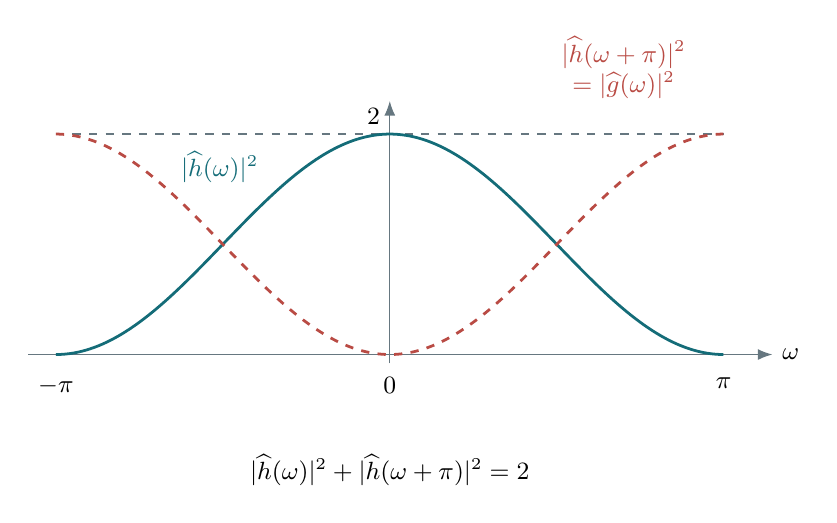
\begin{tikzpicture}[x=1.35cm,y=1.4cm]
\draw[axis] (-3.4,0)--(3.6,0) node[right] {$\omega$};
\draw[axis] (0,-.08)--(0,2.3);
\draw[guide] (-3.14159,2)--(3.14159,2);
\draw[curve,domain=-3.14159:3.14159,samples=201] plot (\x,{2*cos(deg(\x/2))^2});
\draw[signalred,dashed,line width=1pt,domain=-3.14159:3.14159,samples=201] plot (\x,{2*sin(deg(\x/2))^2});
\foreach \x/\lab in {-3.14159/{-\pi},0/0,3.14159/\pi} {\node[below] at (\x,-.12) {$\lab$};}
\node[above left] at (0,2) {$2$};
\node[accent] at (-1.6,1.7) {$|\widehat h(\omega)|^2$};
\node[signalred,align=center] at (2.2,2.6) {$|\widehat h(\omega+\pi)|^2$\\$=|\widehat g(\omega)|^2$};
\node at (0,-1.05) {$|\widehat h(\omega)|^2+|\widehat h(\omega+\pi)|^2=2$};
\end{tikzpicture}
\end{document}
